\documentclass[12pt,a4paper,oneside]{book}

% ============================================================================
% PACKAGES
% ============================================================================
\usepackage[utf-8]{inputenc}
\usepackage[margin=2.5cm]{geometry}
\usepackage{graphicx}
\usepackage{amsmath}
\usepackage{amssymb}
\usepackage{hyperref}
\usepackage{xcolor}
\usepackage{fancyhdr}
\usepackage{array}
\usepackage{booktabs}
\usepackage{listings}
\usepackage{xfrac}
\usepackage{tikz}
\usepackage{tcolorbox}
\usepackage{setspace}
\usepackage{soul}
\usepackage{natbib}
\usepackage{caption}
\usepackage{subcaption}
\usepackage{float}
\usepackage{verbatim}

% ============================================================================
% CUSTOM COLORS
% ============================================================================
\definecolor{darkblue}{rgb}{0.0, 0.2, 0.4}
\definecolor{lightblue}{rgb}{0.8, 0.9, 1.0}
\definecolor{darkgreen}{rgb}{0.1, 0.4, 0.2}
\definecolor{lightgreen}{rgb}{0.9, 1.0, 0.9}
\definecolor{darkred}{rgb}{0.6, 0.0, 0.0}

% ============================================================================
% HYPERLINK SETUP
% ============================================================================
\hypersetup{
    colorlinks=true,
    linkcolor=darkblue,
    urlcolor=darkblue,
    citecolor=darkgreen,
    bookmarksnumbered=true,
    pdfstartview={FitH}
}

% ============================================================================
% HEADER & FOOTER
% ============================================================================
\pagestyle{fancy}
\fancyhf{}
\fancyhead[L]{\small MS Robotics Research Plan}
\fancyhead[R]{\small mAhsanZafar}
\fancyfoot[C]{\thepage}
\renewcommand{\headrulewidth}{0.5pt}

% ============================================================================
% DOCUMENT START
% ============================================================================
\begin{document}

% ============================================================================
% TITLE PAGE
% ============================================================================
\begin{titlepage}
    \centering
    \vspace*{2cm}
    
    {\Huge \textbf{\textcolor{darkblue}{Human-in-the-Loop Cobot Supervision}}}
    
    \vspace{0.5cm}
    {\Huge \textbf{\textcolor{darkblue}{via AR and Natural Language Interfaces}}}
    
    \vspace{2cm}
    {\Large \textbf{MS Robotics Research Proposal}}
    
    \vspace{1.5cm}
    {\Large Muhammad Ahsan Zafar}
    
    \vspace{0.5cm}
    {\normalsize \textit{mAhsanZafar}}
    
    \vspace{2cm}
    
    \vspace{2cm}
    {\large \textbf{Research Direction}}
    
    {\normalsize Direct evolution of voice-controlled AR robotics with IoT integration}
    
    \vspace{1.5cm}
    {\normalsize \today}
    
    \vfill
\end{titlepage}

% ============================================================================
% TABLE OF CONTENTS
% ============================================================================
\tableofcontents
\newpage

% ============================================================================
% CHAPTER 1: RESEARCH OVERVIEW
% ============================================================================
\chapter{Research Overview}

\section{Problem Statement}

Industrial collaborative robots (cobots) currently operate with significant limitations in human supervision:

\begin{itemize}
    \item \textbf{Limited Visualization}: Operators rely on 2D screens and single-angle cameras
    \item \textbf{Complex Interfaces}: Teach pendants and specialized software require extensive training
    \item \textbf{Safety Bottlenecks}: Manual monitoring leads to delayed interventions
    \item \textbf{Cognitive Overload}: Operators struggle with multi-modal information integration
\end{itemize}

\subsection{Research Objective}

Develop an integrated \textcolor{darkblue}{\textbf{AR + NLP-based supervision system}} enabling operators to monitor, control, and intervene with cobots using:
\begin{enumerate}
    \item Real-time natural language commands
    \item Spatial augmented reality visualization
    \item Context-aware safety monitoring
    \item Predictive intervention prompts
\end{enumerate}

\section{Novelty and Impact}

\begin{tcolorbox}[colback=lightblue, colframe=darkblue, title=Key Innovations]
\begin{itemize}
    \item \textbf{Real-time AR visualization} of cobot state, trajectory, and environmental awareness
    \item \textbf{Natural language command execution} converting voice to high-level robot tasks
    \item \textbf{Context-aware intervention prediction} anticipating when human input is needed
    \item \textbf{Safety-critical integration} for manufacturing, healthcare, and inspection
\end{itemize}
\end{tcolorbox}

\subsection{Expected Impact}
\begin{description}
    \item[Industrial Impact] Reduce operator training time by 40-60\%, increase cobot uptime
    \item[Economic Impact] Enable small/medium manufacturers to adopt collaborative robots
    \item[Scientific Impact] Advances in HRI, AR-based teleoperation, and industrial NLU
    \item[Safety Impact] Formal verification of AR-guided commands against safety constraints
\end{description}

\newpage

% ============================================================================
% CHAPTER 2: TECHNICAL ARCHITECTURE
% ============================================================================
\chapter{Technical Architecture}

\section{System Overview}

\subsection{Three-Tier Stack}

\begin{figure}[H]
\centering
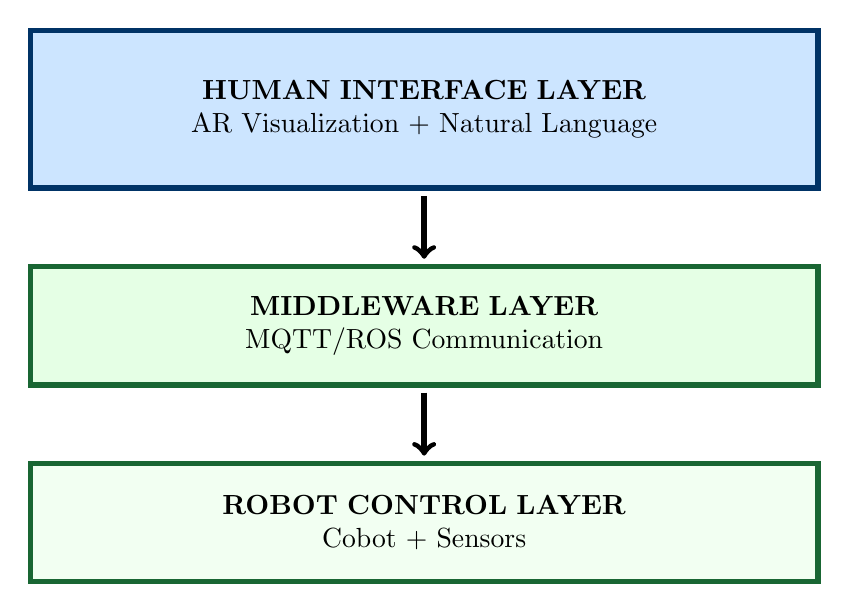
\begin{tikzpicture}[scale=1.0]
    % Layer 1
    \draw[fill=lightblue, draw=darkblue, line width=2pt] (0, 6) rectangle (10, 8);
    \node[text width=9cm, align=center] at (5, 7) {\textbf{HUMAN INTERFACE LAYER} \\ AR Visualization + Natural Language};
    
    % Arrow
    \draw[->, line width=2pt] (5, 5.9) -- (5, 5.1);
    
    % Layer 2
    \draw[fill=lightgreen, draw=darkgreen, line width=2pt] (0, 3.5) rectangle (10, 5);
    \node[text width=9cm, align=center] at (5, 4.25) {\textbf{MIDDLEWARE LAYER} \\ MQTT/ROS Communication};
    
    % Arrow
    \draw[->, line width=2pt] (5, 3.4) -- (5, 2.6);
    
    % Layer 3
    \draw[fill=lightgreen!50, draw=darkgreen, line width=2pt] (0, 1) rectangle (10, 2.5);
    \node[text width=9cm, align=center] at (5, 1.75) {\textbf{ROBOT CONTROL LAYER} \\ Cobot + Sensors};
    
\end{tikzpicture}
\caption{Three-Tier System Architecture}
\label{fig:architecture}
\end{figure}

\subsection{Component Details}

\subsubsection{Human Interface Layer (Android/Kotlin)}
\begin{itemize}
    \item ARCore-based spatial visualization
    \item Real-time speech recognition \& NLU
    \item AR annotations: robot state, safety zones, predicted paths
    \item Gesture-based secondary controls
\end{itemize}

\subsubsection{Middleware Layer (MQTT/ROS 2)}
\begin{itemize}
    \item ThingESP MQTT broker for IoT communication
    \item ROS 2 node integration for standardized robotics
    \item Real-time telemetry synchronization (<50ms latency)
    \item Command queuing and priority management
\end{itemize}

\subsubsection{Robot Control Layer}
\begin{itemize}
    \item UR/ABB/Stäubli cobot integration
    \item Multi-sensor fusion (RGB-D, lidar, force/torque)
    \item Motion planning and trajectory execution
    \item Safety monitoring and constraint checking
\end{itemize}

\section{Core Technologies}

Your existing work provides the foundation:

\begin{table}[H]
\centering
\begin{tabular}{|l|l|l|}
\hline
\textbf{Component} & \textbf{Source Project} & \textbf{Usage} \\
\hline
AR Visualization & VoiceControlled-AR-Robot & Foundation framework \\
Voice Commands & voice-controlled-AI-assistant & NLU + intent parsing \\
Multi-modal AI & omnibrain-ai-system & Knowledge integration \\
IoT Patterns & Home automation projects & Device communication \\
ML Prediction & CardioRiskML & Anomaly detection \\
\hline
\end{tabular}
\caption{Technology Stack Mapping}
\label{tab:tech_stack}
\end{table}

\newpage

% ============================================================================
% CHAPTER 3: RESEARCH CONTRIBUTIONS
% ============================================================================
\chapter{Research Contributions}

\section{Contribution 1: Adaptive AR Context Rendering}

\subsection{Challenge}
Real-time rendering of 6-DOF robot pose, point clouds, safety zones, and predicted trajectories in AR.

\subsection{Research Questions}
\begin{enumerate}
    \item How to efficiently stream multi-modal sensor data to AR client?
    \item What AR visualization grammar best supports operator comprehension?
    \item What annotation density maximizes decision quality without cognitive overload?
\end{enumerate}

\subsection{Methodology}
\begin{itemize}
    \item Design parametric AR visualization system
    \item Implement spatial indexing for efficient scene updates
    \item Conduct HCI studies: operator performance vs. visualization complexity
    \item Benchmark latency: target <50ms AR-to-robot sync
\end{itemize}

\subsection{Expected Deliverables}
\begin{tcolorbox}[colback=lightgreen, colframe=darkgreen]
\begin{itemize}
    \item ARCore rendering pipeline with custom shaders
    \item Publication: ``Adaptive AR Visualization for Human-Robot Supervision''
    \item Open-source ARCore extensions for robot telemetry
    \item HCI study dataset with 30+ operators
\end{itemize}
\end{tcolorbox}

---

\section{Contribution 2: Intent Recognition \& Task Grounding}

\subsection{Challenge}
Converting natural language commands into executable robot task graphs.

\subsection{Research Questions}
\begin{enumerate}
    \item How to ground NL in cobot action space?
    \item How to resolve ambiguity with interactive clarification?
    \item Can robots learn new tasks from single human demonstration + language?
\end{enumerate}

\subsection{Methodology}
\begin{itemize}
    \item Fine-tune LLM (Google Gemini) on industrial domain
    \item Semantic parsing: NL $\rightarrow$ task graphs
    \item Few-shot learning from human demonstration
    \item Adversarial testing: out-of-domain robustness
\end{itemize}

\subsection{Expected Deliverables}
\begin{tcolorbox}[colback=lightgreen, colframe=darkgreen]
\begin{itemize}
    \item Domain-specific NLU model ($\geq$100 industrial tasks)
    \item Publication: ``Grounded Natural Language Understanding for Robot Task Specification''
    \item Annotation dataset: 2,000+ NL-task pairs
    \item Interactive task learning interface
\end{itemize}
\end{tcolorbox}

---

\section{Contribution 3: Context-Aware Intervention Prediction}

\subsection{Challenge}
Predicting when human intervention is needed \textit{before} failures occur.

\subsection{Research Questions}
\begin{enumerate}
    \item What sensor signals indicate necessary intervention?
    \item Can we predict with high precision without false alarms?
    \item How does prediction accuracy vary by operator expertise?
\end{enumerate}

\subsection{Methodology}
\begin{itemize}
    \item Multi-modal anomaly detection: LSTMs + sensor fusion
    \item Temporal modeling of robot state sequences
    \item User studies: passive monitoring vs. predicted alerts
    \item Calibration: task-dependent intervention thresholds
\end{itemize}

\subsection{Expected Deliverables}
\begin{tcolorbox}[colback=lightgreen, colframe=darkgreen]
\begin{itemize}
    \item Multi-modal anomaly detector (F1 score $> 0.85$)
    \item Publication: ``Predictive Intervention Prompts in Human-Robot Collaboration''
    \item Real-time monitoring dashboard
    \item Sensor dataset: 100+ hours cobot telemetry
\end{itemize}
\end{tcolorbox}

---

\section{Contribution 4: Safety \& Compliance Certification}

\subsection{Challenge}
Ensuring AR-guided commands comply with industrial safety standards (ISO/TS 15066, ANSI/RIA).

\subsection{Research Questions}
\begin{enumerate}
    \item How to formally verify trajectory safety?
    \item What safety guarantees can AR provide?
    \item How to audit all interventions for compliance?
\end{enumerate}

\subsection{Methodology}
\begin{itemize}
    \item Formal verification: model-checking against constraints
    \item FMEA: Failure Mode \& Effects Analysis
    \item Immutable audit logging (blockchain-inspired)
    \item User study: safety with vs. without AR guidance
\end{itemize}

\subsection{Expected Deliverables}
\begin{tcolorbox}[colback=lightgreen, colframe=darkgreen]
\begin{itemize}
    \item Formal verification toolkit for cobot trajectories
    \item Publication: ``Safety Certification of AR-Mediated Robot Control''
    \item Compliance documentation (ISO 13849-1)
    \item Audit logging system
\end{itemize}
\end{tcolorbox}

\newpage

% ============================================================================
% CHAPTER 4: EXPERIMENTAL VALIDATION
% ============================================================================
\chapter{Experimental Validation Roadmap}

\section{Phase 1: Foundation (Months 1-4)}

\begin{table}[H]
\centering
\begin{tabular}{|l|p{7cm}|}
\hline
\textbf{Task} & \textbf{Description} \\
\hline
ROS Integration & Setup UR/ABB cobot simulator in Gazebo \\
AR Telemetry & Implement ARCore $\leftrightarrow$ cobot communication \\
NLU Module & Build intent classifier on 10 core tasks \\
Baseline & Establish traditional teach pendant baseline \\
\hline
\end{tabular}
\caption{Phase 1 Milestones}
\end{table}

\section{Phase 2: Integration (Months 5-8)}

\begin{itemize}
    \item Voice $\rightarrow$ NLU $\rightarrow$ task execution pipeline
    \item AR visualization of robot + safety zones + trajectories
    \item Deploy anomaly detection model
    \item Internal usability testing (lab environment)
\end{itemize}

\section{Phase 3: Evaluation (Months 9-12)}

\subsection{User Study Design}

\begin{table}[H]
\centering
\begin{tabular}{|l|l|}
\hline
\textbf{Parameter} & \textbf{Specification} \\
\hline
Task Types & Pick-and-place, assembly, inspection \\
Operator Levels & Novice, intermediate, expert \\
Conditions & Traditional interface vs. AR+NLP \\
Metrics & Completion time, safety, cognitive load \\
Participants & 30+ professional operators \\
\hline
\end{tabular}
\caption{User Study Specification}
\end{table}

\section{Phase 4: Real-World Deployment (Months 13-18)}

\begin{enumerate}
    \item Partner with industry manufacturers
    \item Field trials in production environment
    \item Safety certification pathway
    \item Thesis writing and publication strategy
\end{enumerate}

\newpage

% ============================================================================
% CHAPTER 5: DATASETS AND BENCHMARKS
% ============================================================================
\chapter{Datasets \& Benchmarks}

\section{Dataset 1: NL-Task Grounding}

\begin{lstlisting}[language=json, caption=Example NL-Task Pair]
{
  "nl_command": "Move the blue part to assembly bin with 20% force",
  "task_graph": {
    "subtasks": [
      {"name": "detect_object", "color": "blue"},
      {"name": "move_to_object"},
      {"name": "grasp", "force_threshold": 20},
      {"name": "move_to_location", "target": "assembly_bin"},
      {"name": "release"}
    ]
  },
  "robot_state": {...},
  "executed_trajectory": {...}
}
\end{lstlisting}

\section{Dataset 2: Anomaly Detection Benchmark}

\begin{itemize}
    \item Multi-modal sensor logs: vision, force/torque, joint angles, safety violations
    \item Labels: normal operation, collision, slip, obstruction, etc.
    \item Volume: 100+ hours (simulator + real cobot)
    \item Modalities: 4+ sensor types per sample
\end{itemize}

\section{Dataset 3: AR Visualization Preferences}

\begin{itemize}
    \item Video comparisons of AR rendering styles
    \item Operator rankings by task and expertise
    \item Eye-tracking data (saliency analysis)
    \item Cognitive load assessment (NASA TLX)
\end{itemize}

\newpage

% ============================================================================
% CHAPTER 6: IMPLEMENTATION DETAILS
% ============================================================================
\chapter{Implementation Details}

\section{Technology Stack}

\begin{table}[H]
\centering
\begin{tabular}{|l|l|}
\hline
\textbf{Component} & \textbf{Technology} \\
\hline
Frontend & Kotlin (Android) + ARCore + ML Kit \\
Backend & Python + ROS 2 + FastAPI \\
Communication & MQTT (ThingESP) + gRPC \\
Robot Integration & UR Script, ABB RAPID, Gazebo \\
ML/AI & TensorFlow/PyTorch + HuggingFace \\
Safety Verification & TLA+, Uppaal, model-checker \\
\hline
\end{tabular}
\caption{Complete Technology Stack}
\end{table}

\section{Repository Structure}

\begin{verbatim}
human-cobot-supervision/
├── android-ar-client/              # Kotlin, ARCore frontend
├── robot-control-backend/          # Python, ROS 2 backend
├── nlu-intent-classifier/          # Transformers fine-tuning
├── anomaly-detector/               # ML models, sensor fusion
├── safety-verification/            # Formal methods tools
├── datasets/                       # NL-task, telemetry, prefs
├── experiments/                    # User studies, benchmarks
├── docs/                          # Architecture, papers
└── docker-compose.yml             # Full stack deployment
\end{verbatim}

\section{Development Timeline}

\begin{table}[H]
\centering
\begin{tabular}{|c|l|l|}
\hline
\textbf{Month} & \textbf{Phase} & \textbf{Deliverables} \\
\hline
1-2 & Literature Review & 50+ papers surveyed \\
3-4 & Architecture Design & System design documents \\
5-6 & Prototype MVP & Basic AR + voice integration \\
7-8 & NLU Integration & 50-task NLU model \\
9-10 & Anomaly Detection & ML model training complete \\
11-12 & User Studies & Phase 1 evaluation done \\
13-14 & Field Trials & Partner deployment \\
15-16 & Analysis & 2-3 papers submitted \\
17-18 & Thesis Writing & Final thesis completion \\
\hline
\end{tabular}
\caption{18-Month Development Timeline}
\end{table}

\newpage

% ============================================================================
% CHAPTER 7: RISK MITIGATION
% ============================================================================
\chapter{Risk Mitigation \& Contingencies}

\begin{table}[H]
\centering
\begin{tabular}{|p{3cm}|p{5cm}|}
\hline
\textbf{Risk} & \textbf{Mitigation Strategy} \\
\hline
Cobot Access & Use Gazebo simulator (free, open-source) initially \\
NLU Coverage & Start with 50 core tasks, expand iteratively \\
AR Latency & Client-side prediction (dead reckoning) \\
User Recruitment & Partner with robotics labs, industry contacts \\
Safety Certification & Early engagement with standards bodies \\
Publication Pressure & Publish incrementally (3-4 papers min.) \\
\hline
\end{tabular}
\caption{Risk Mitigation Table}
\end{table}

\newpage

% ============================================================================
% CHAPTER 8: IMPACT AND APPLICATIONS
% ============================================================================
\chapter{Impact \& Applications}

\section{Immediate Applications}

\begin{description}
    \item[Manufacturing] Assembly lines, quality inspection, collaborative assembly
    \item[Healthcare] Surgical cobot supervision, sterilization assistance
    \item[Warehousing] Autonomous picking with human oversight
    \item[Construction] Prefabrication, on-site assembly with remote supervision
\end{description}

\section{Economic Impact}

\begin{itemize}
    \item \textbf{40-60\% reduction} in operator training time
    \item \textbf{Increased cobot uptime} via faster problem resolution
    \item \textbf{Market expansion} to SMEs (small/medium enterprises)
    \item \textbf{New product category}: AR-first cobot interfaces
\end{itemize}

\section{Scientific Contributions}

\begin{enumerate}
    \item Advances in human-robot interaction (HRI)
    \item Novel AR-based teleoperation paradigm
    \item Practical safety certification methodology
    \item Industrial NLU dataset and benchmarks (open-source)
\end{enumerate}

\newpage

% ============================================================================
% CHAPTER 9: RELATED WORK
% ============================================================================
\chapter{Related Work \& Positioning}

\section{Competitive Landscape}

\begin{table}[H]
\centering
\begin{tabular}{|l|l|l|l|}
\hline
\textbf{Aspect} & \textbf{Your Work} & \textbf{Competitors} & \textbf{Novel?} \\
\hline
AR Visualization & Custom ARCore + fusion & ROS-RViz (2D) & \checkmark \\
Voice Control & Context-aware NLU & ABB Robotics Studio & \checkmark \\
Prediction & Anomaly-based & Reactive systems & \checkmark \\
Integration & Full-stack AR+NLP & Point solutions & \checkmark \\
\hline
\end{tabular}
\caption{Competitive Analysis}
\end{table}

\section{Publication Venues}

\begin{itemize}
    \item \textbf{Top-tier Robotics}: ICRA, IROS, RSS
    \item \textbf{HCI/AI}: CHI, IUI, UIST
    \item \textbf{Safety-Critical}: HSCC, RTAS
    \item \textbf{AI Applications}: IJCAI, AAAI
    \item \textbf{Domain-Specific}: IROS HRI workshop, CoRL
\end{itemize}

\newpage

% ============================================================================
% CHAPTER 10: NEXT STEPS
% ============================================================================
\chapter{Recommended Next Steps}

\section{Immediate Actions (Week 1-2)}

\begin{enumerate}
    \item Start literature review: 50+ papers on AR robotics, grounding, HRI, anomaly detection
    \item Join robotics communities: ROS, IEEE, ACM SIGCHI
    \item Identify potential industry partners
\end{enumerate}

\section{Short-term (Weeks 3-4)}

\begin{enumerate}
    \item Build MVP prototype:
    \begin{itemize}
        \item ARCore $\leftrightarrow$ mock cobot state
        \item 10 basic voice commands
        \item Render robot + safety zones
    \end{itemize}
    \item Set up development environment (ROS 2, Gazebo)
\end{enumerate}

\section{Medium-term (Months 2-3)}

\begin{enumerate}
    \item Finalize industry partnerships
    \item Complete research proposal for funding
    \item Submit to: NSF REU, DoD Manufacturing grants, university startups
\end{enumerate}

\section{Long-term (Months 4-18)}

Follow the phased roadmap outlined in previous chapters.

\newpage

% ============================================================================
% CHAPTER 11: APPENDIX
% ============================================================================
\appendix

\chapter{Key References}

\begin{thebibliography}{99}

\bibitem{ISO15066} ISO/TS 15066:2016, \textit{Robots and robotic devices -- Collaborative robots -- Safety requirements for design, performance and operation}.

\bibitem{ANSI} ANSI/RIA R15.06, \textit{Industrial Robots and Robot Systems -- Safety Requirements}.

\bibitem{ARCore} Google AR Core Documentation, \url{https://developers.google.com/ar/discover}

\bibitem{ROS2} ROS 2 Official Documentation, \url{https://docs.ros.org/en/rolling/}

\bibitem{Gazebo} Gazebo Robotics Simulator, \url{https://gazebosim.org/}

\bibitem{Gemini} Google Gemini API Documentation, \url{https://ai.google.dev/gemini-api}

\end{thebibliography}

\chapter{Author Information}

\begin{tcolorbox}[colback=lightblue, colframe=darkblue]
\textbf{Name}: Muhammad Ahsan Zafar\\
\textbf{GitHub}: \url{https://github.com/mAhsanZafar}\\
\textbf{Research Interests}: AR Robotics, Natural Language Understanding, Human-Robot Interaction, IoT Systems\\
\textbf{Education}: BS Information \& Communication Engineering (The Islamia University of Bahawalpur)\\
\textbf{Experience}: Machine Learning, Voice-Controlled Systems, IoT Automation, Android Development
\end{tcolorbox}

\vfill

\begin{center}
\textit{Document created: \today}\\
\textit{Research Plan Status: Active}
\end{center}

\end{document}
